\noindent

\includegraphics[height=1.25cm]{images/pictograms/replication}
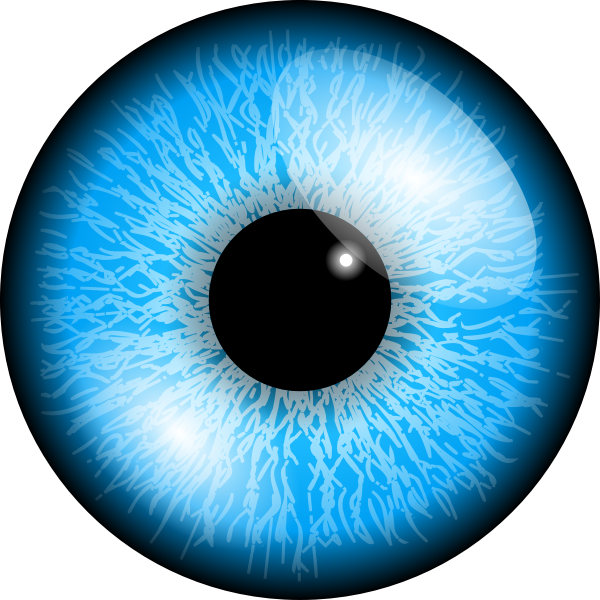
\includegraphics[height=1.25cm]{images/pictograms/visualisation}

\includegraphics[height=1.25cm]{images/pictograms/benchmark}

\includegraphics[height=1.25cm]{images/pictograms/under_construction}

\includegraphics[height=1.25cm]{images/pictograms/tools}

\includegraphics[height=1.25cm]{images/pictograms/FEM}

\includegraphics[height=1.25cm]{images/pictograms/FDM}

\includegraphics[height=1.25cm]{images/pictograms/3d}

\includegraphics[height=1.25cm]{images/pictograms/nonlinear}

\includegraphics[height=1.25cm]{images/pictograms/paraview}

%%%%%%%%%%%%%%%%%%%%%%%%%%%%%%%%%%%%%%%%%%%%%%%%%%%%%%%%%%%%%%%%%%%%%%%%%%%%%%%%%%%%%%%%%%%%%%%%%%%

\begin{flushright} {\tiny {\color{gray} python\_codes/fieldstone\_171/text.tex}} \end{flushright}

%\lstinputlisting[language=bash,basicstyle=\small]{python_codes/template_keywords.key}

\par\noindent\rule{\textwidth}{0.4pt}

\begin{center}
\inpython
{\small Code: \url{https://github.com/cedrict/fieldstone/tree/master/python_codes/fieldstone_171}}
\end{center}

\par\noindent\rule{\textwidth}{0.4pt}

{\sl This stone was developed in collaboration with L. van de Wiel}. \index{contributors}{L. van de Wiel}

\par\noindent\rule{\textwidth}{0.4pt}

Last revision: March. 23th, 2025.

\par\noindent\rule{\textwidth}{0.4pt}

%%%%%%%%%%%%%%%%%%%%%%%%%%%%%%%%%%%%%%%%%%%%%%%%%%%%%%%%%%%%%%%%%%%%%%%%%%%%%%%%%%%%%%%%%%%%%%%%%%%


\url{https://en.wikipedia.org/wiki/Reaction-diffusion_system}

The systematic generation of porous geometries is based on a special treatment, outlined in
the rest of this section, of a class of solutions to the Gray–Scott reaction–diffusion system
of equations given by
\begin{eqnarray}
\frac{\partial U}{\partial t} &=& D_u \vec\nabla^2 U - UV^2 + F(1-U) \nn\\
\frac{\partial V}{\partial t} &=& D_v \vec\nabla^2 V + UV^2 - (F+k)V 
\end{eqnarray}
where $D_u$ and $D_v$ are diffusion coefficients associated with the species concentration $U$and $V$
$k$ is the dimensionless rate constant of the second reaction (also commonly called the `kill 
parameter') and $F$ is the dimensionless feed rate.
Often periodic boundary conditions are used. 

\textcite{gama23} (2023) rely on these equations to generate porous geometries 
and the following values of $D_u,D_v,f,k$ are used:

\begin{center}
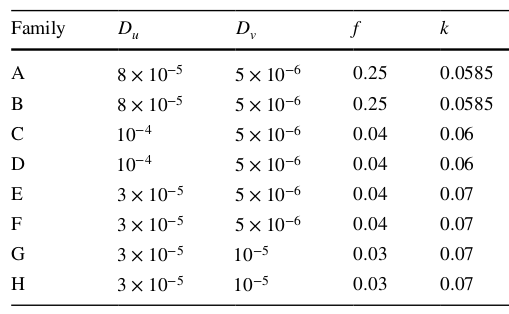
\includegraphics[width=6cm]{python_codes/fieldstone_171/images/gama01}
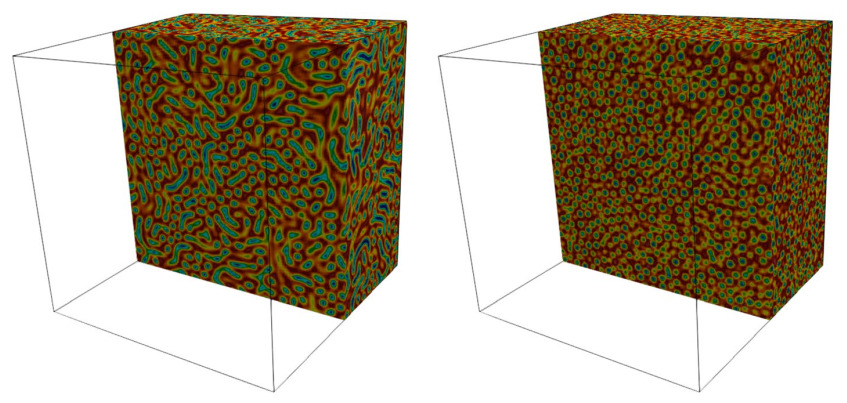
\includegraphics[width=9cm]{python_codes/fieldstone_171/images/gama02}\\
{\captionfont Iso-surfaces for solutions to the reaction-diffusion system 
for two set of parameters $\{D_u,D_v,F,k\}$, the parameters on the figure on 
the left(right) correspond to family A/B(C/D) in the table. The solutions were
obtained on a cube of length $L=192$.}
\end{center}

In the articles the authors use spherical initial distributions given by:
\begin{eqnarray}
U(r,\theta,\phi) &=& H_e(r-r_c) +\frac12 (1-H_e(r-r_c)) + 0.01 \cdot {\cal U}_{[0,1]} \nn\\
V(r,\theta,\phi) &=& \frac14 (1-H_e(r-r_c)) + 0.01 \cdot {\cal U}_{[0,1]}
\end{eqnarray}
where $H_e$ is the Heaviside step function, ${\cal U}_{[0,1]}$ is a random variable sourced from a 
uniform distribution defined between $[0,1]$, and $(r,\theta,\phi)$ are spherical coordinates centered at
the cube center, and $r_c$ is a constant (5 or 7).
The equations are solved numerically via a finite difference scheme on a cube of size $L$
with periodic boundary conditions. As time evolves, the patterns generated by
the solutions reveal a class of solutions whose iso-surfaces are reminiscent of the internal
boundaries encountered on porous media as shown in the figure above.




Grab code from f130

relevant \cite{pear93}

%%%%%%%%%%%%%%%%%%%%%%%%%%%%%%%%%%%%%%%%%%%%%%%
\section*{Lkas van de Wiel's approach}

Lukas says:
\begin{verbatim}
 I used a resolution of 4800x4800 but that is quite large.
1000x1000 will most likely get you fine results.
dudt = DU * Lu +  FEED * (1.0 - u) - u*v^2
dvdt = DV * Lv - (FEED + KILL)* v  + u*v^2
with Lu and Lv the Laplacian of u and v
For the pumice mesh:
#define DU   0.000004
#define DV   0.000002
#define FEED   0.035
#define KILL   0.0575
Initial conditions:
u = 1, with random seed squares of a random size (edge length) 
between 11 and 60 and a value between 0.5 and 1
v = 0, with random seed squares of a random size (edge length) 
between 11 and 60 and a value between 0 and 0.25
The squares in u and those in v are independent from each other
if you reduce the resolution, it would make sense to reduce the seed size correspondingly.
I applied a thousand of these seeds in u and a thousand in v.
Time stepping:
I use RK4 timesteps, with
#define DT   0.001
#define N_PLOTS   100
#define N_TIMESTEPS_BETWEEN_PLOTS   100000
So I got a plot every 0.001 * 100000 = 100
so plot u000012.jpg is after time 1200.
For your validation, I added some of those plots of U
I solved in on a GPU, which did this in about a day, on 4800x4800.
Adaptive timestepping will probably be an improvement near the end,  
because the sharp edges around the seed squares will have gone.
It could no doubt be improved by turning the hard edges seed squares into 
soft edges seed blobs/gaussians, but then the smoothness of the patterns
depends on the parameters of Du and Dv, and needed something that works universally, for consistency.
(If you reduce Du and Dv, you well get a more fine grained pattern, as if zoomed out more)
If you want to create the full pattern range like the background of my poster, you need let F and K change.
I let K change with x, and F with y, but that was because of the orientation I wished on the poster,
you can do just as well the other way around.
Letting both vary between 0 and 0.1 will give you the full spectrum.
Method of lines - no particular attention to nonlinearities. 
\end{verbatim}

\begin{center}
\includegraphics[width=5.6cm]{python_codes/fieldstone_171/images/u000000.jpg}
\includegraphics[width=5.6cm]{python_codes/fieldstone_171/images/u000001.jpg}
\includegraphics[width=5.6cm]{python_codes/fieldstone_171/images/u000003.jpg}\\
\includegraphics[width=5.6cm]{python_codes/fieldstone_171/images/u000007.jpg}
\includegraphics[width=5.6cm]{python_codes/fieldstone_171/images/u000012.jpg}
\includegraphics[width=5.6cm]{python_codes/fieldstone_171/images/u000020.jpg}
\end{center}

%%%%%%%%%%%%%%%%%%%%%%%%%%%%%%%%%%%%%%%%%%%%%%%%%%%%%%%%%%%%%%%%%%%%%%%%%%%%%%%%%%%%%
\section*{A word about methods}

We are dealing with a set of coupled nonlinear PDEs to which there are no analytical solution.
We must then solve them by means of a numerical method. 
Obviously a Finite Difference of Finite Element approach could be envisaged. The main difficulty then
would be (as discussed in \stone~130) how to deal with the nonlinear terms. Also, based on 
the results presented above by Lukas it appears that a high resolution should be envisaged
of (at least?) $1000\times 1000$ nodes. This would yield *very* large linear systems to be 
solved hundreds/thousands of time.
Keeping this in mind we therefore decide to resort to the method of lines as in \stone~157.

We discretise the Laplace operators as follows:
\[
\vec\nabla^2 u \simeq 
\frac{u_{i-1,j,k}-2u_{i,j,k}+u_{i+1,j,k}}{h_x^2} + 
\frac{u_{i-1,j,k}-2u_{i,j,k}+u_{i+1,j,k}}{h_y^2} + 
\frac{u_{i,j,k-1}-2u_{i,j,k}+u_{i,j,k+1}}{h_z^2} 
\]
so that the PDEs can be discretised in space at a node $i$ as follows:
\begin{eqnarray}
\frac{\partial u_{i,j,k}}{\partial t} &=& D_u 
\left(
\frac{u_{i-1,j,k}-2u_{i,j,k}+u_{i+1,j,k}}{h_x^2} + 
\frac{u_{i-1,j,k}-2u_{i,j,k}+u_{i+1,j,k}}{h_y^2} + 
\frac{u_{i,j,k-1}-2u_{i,j,k}+u_{i,j,k+1}}{h_z^2} 
\right)
- u_{i,j,k}v_{i,j,k}^2 + F(1-u_{i,j,k}) 
\nn\\
\frac{\partial v_{i,j,k}}{\partial t} &=& D_v 
\left(
\frac{v_{i-1,j,k}-2v_{i,j,k}+v_{i+1,j,k}}{h_x^2} + 
\frac{v_{i-1,j,k}-2v_{i,j,k}+v_{i+1,j,k}}{h_y^2} + 
\frac{v_{i,j,k-1}-2v_{i,j,k}+v_{i,j,k+1}}{h_z^2} 
\right)
+ u_{i,j,k}v_{i,j,k}^2 - (F+k)v_{i,j,k}
\end{eqnarray}










